\section{Home Server Deployment}
\label{research:HomeServerDeployment}
Building a tool that aims to recreate and improve on the functionality found by market leading platforms built by huge multinational corporations was bound to come with some challenges. Often these would be down to a lack of human time (being just me working on this within the scope of an EPQ), some are limitations on the skill I have and can gain over this year, however some are financially constraining and tools which would simplify or even eliminate challenges aren't available to me. Getting my project hosted online was one such challenge.

From my prior research Id learnt that platforms such as OneNote have two main challenges associated with making their platforms functional to users around the world, firstly they need to deliver a client to the user that can represent the information they have stored and allow them to take new notes, secondly they need a backend "API" to allow each client to  interface with the large databases back at OneNote headquarters (in practice this is on Azure - Microsoft's 'cloud' services platform), this API enables clients to access the pre-existing notes, to save new copies, login to accounts etc. 

At first I want to try and solve two birds with one stone and deploy a server from my house that can send a user the code to display the website when requested and can respond to that codes request to interact with my database (also running on the same server). The device I have chosen for this is a Raspberry pi 5 due to its low power usage, ability to connect to external storage drives (for database records and backup) and importantly low power usage which is both better for the environment and cheaper to operate compared to leaving a more conventional computer powered for the duration of my project. 

With a compute device chosen I next needed to choose an operating system. After some research I found that most experts online recommended sticking with the OS Linux 'flavour' developed by the same company as the raspberry Pi's creator due to its excellent reliability, great compatibility and ease of use. This left me with one final decision to make before choosing: a standard system environment or a 'headless' Lite install. While the former option is more conventional with a desktop, icons and buttons the user can click on with a mouse, the latter has only a 'terminal' environment. Put simply this is like going back to computers from the 70s, a traditional text only interface where I can input commands and see results also in text. Whilst this may seem a strange choice when the GUI options are so much more familiar, headless installs come with three main benefits: lower system resource usage to display the desktop etc and easier ability to remotely control the computer from anywhere. As I expect my project will already be pushing the Pi this was crucial and the ability to control the device from anywhere is a common professional capability, and in this process I want to make my software and systems as professional as possible.

Having selected Raspbian Lite as my device OS I took my Sd card and used my laptop to flash the card with a copy , using this time to prefill some basic details such as username and password (so that I can connect to the device later), time zone (a very important detail when networking devices) and assigning a static IP address from my router panel (this makes connecting much easier later).

\begin{figure}[H]
    \centering
    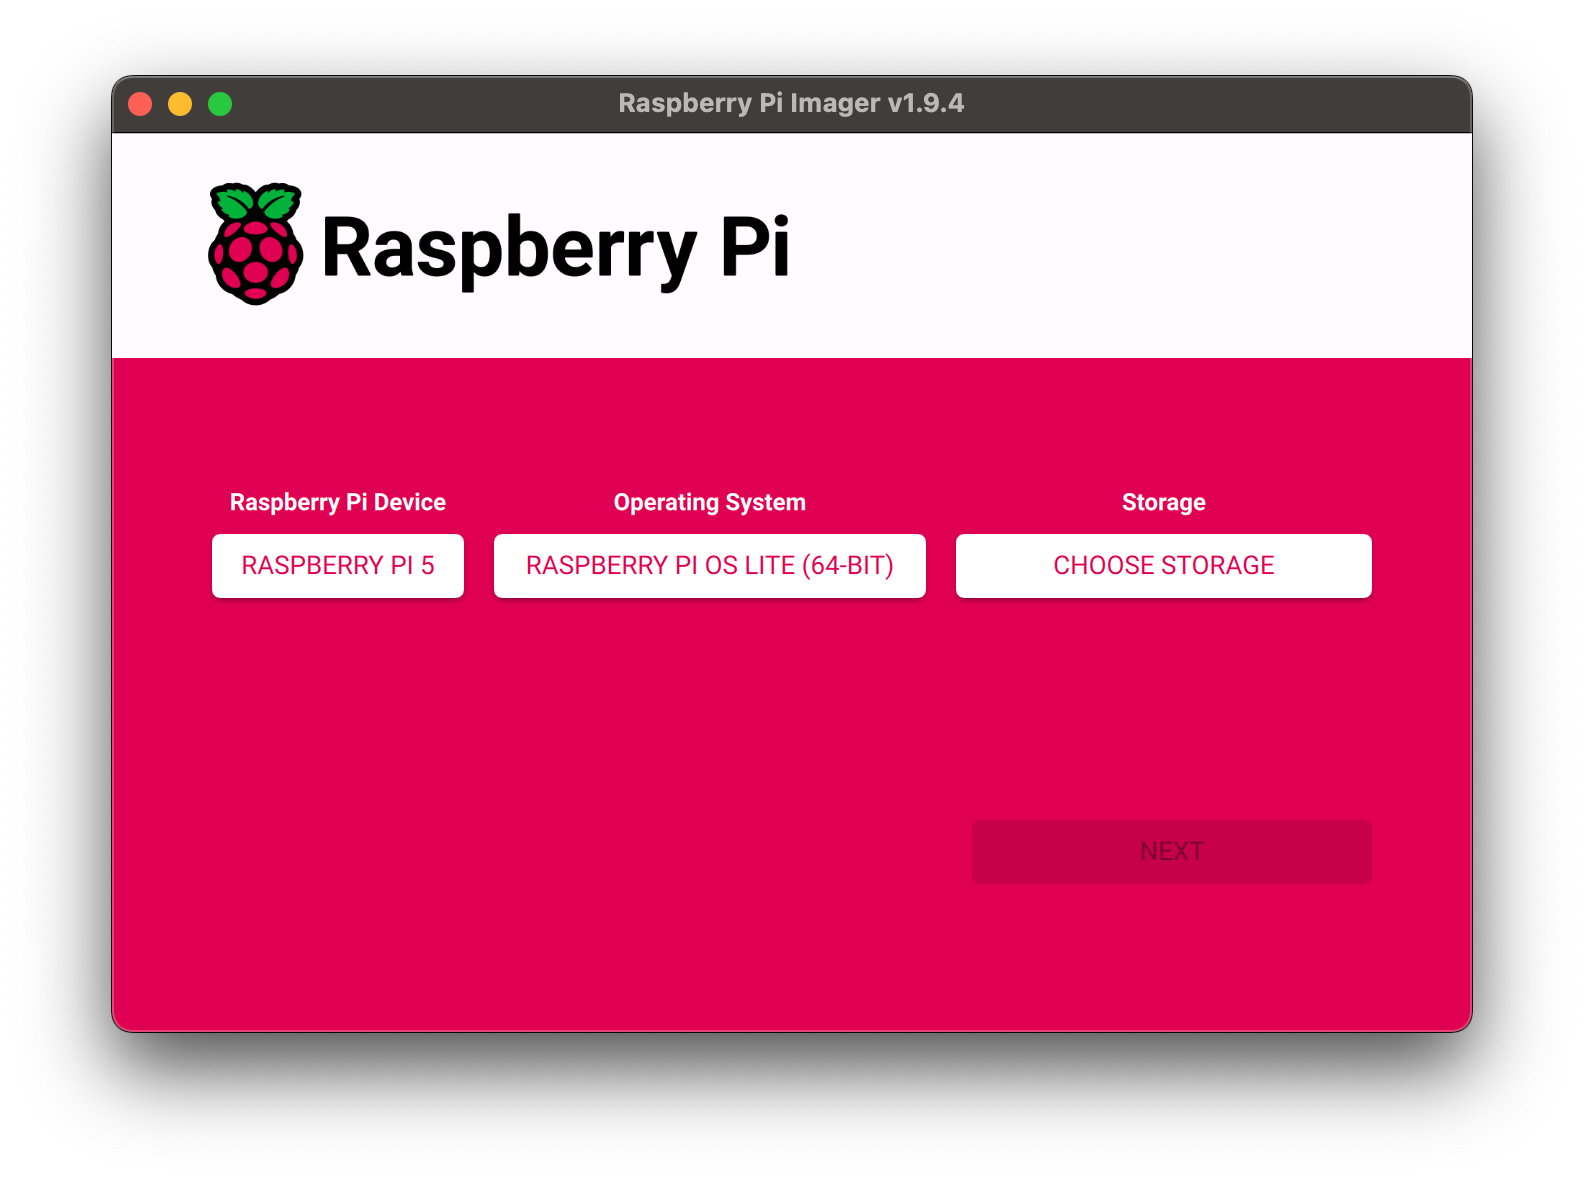
\includegraphics[width=0.8\textwidth]{Research/31_HomeServerDeployment/media/RPIInstallation.png}
    \caption{Raspberry Pi installation media tool}
\end{figure}

I inserted the card into the pi and powered it on, after waiting for the initialisation sequence to complete I could now use the terminal application from my MacBook to SSH (secure shell) into the pi and take control. 

\begin{figure}[H]
    \centering
    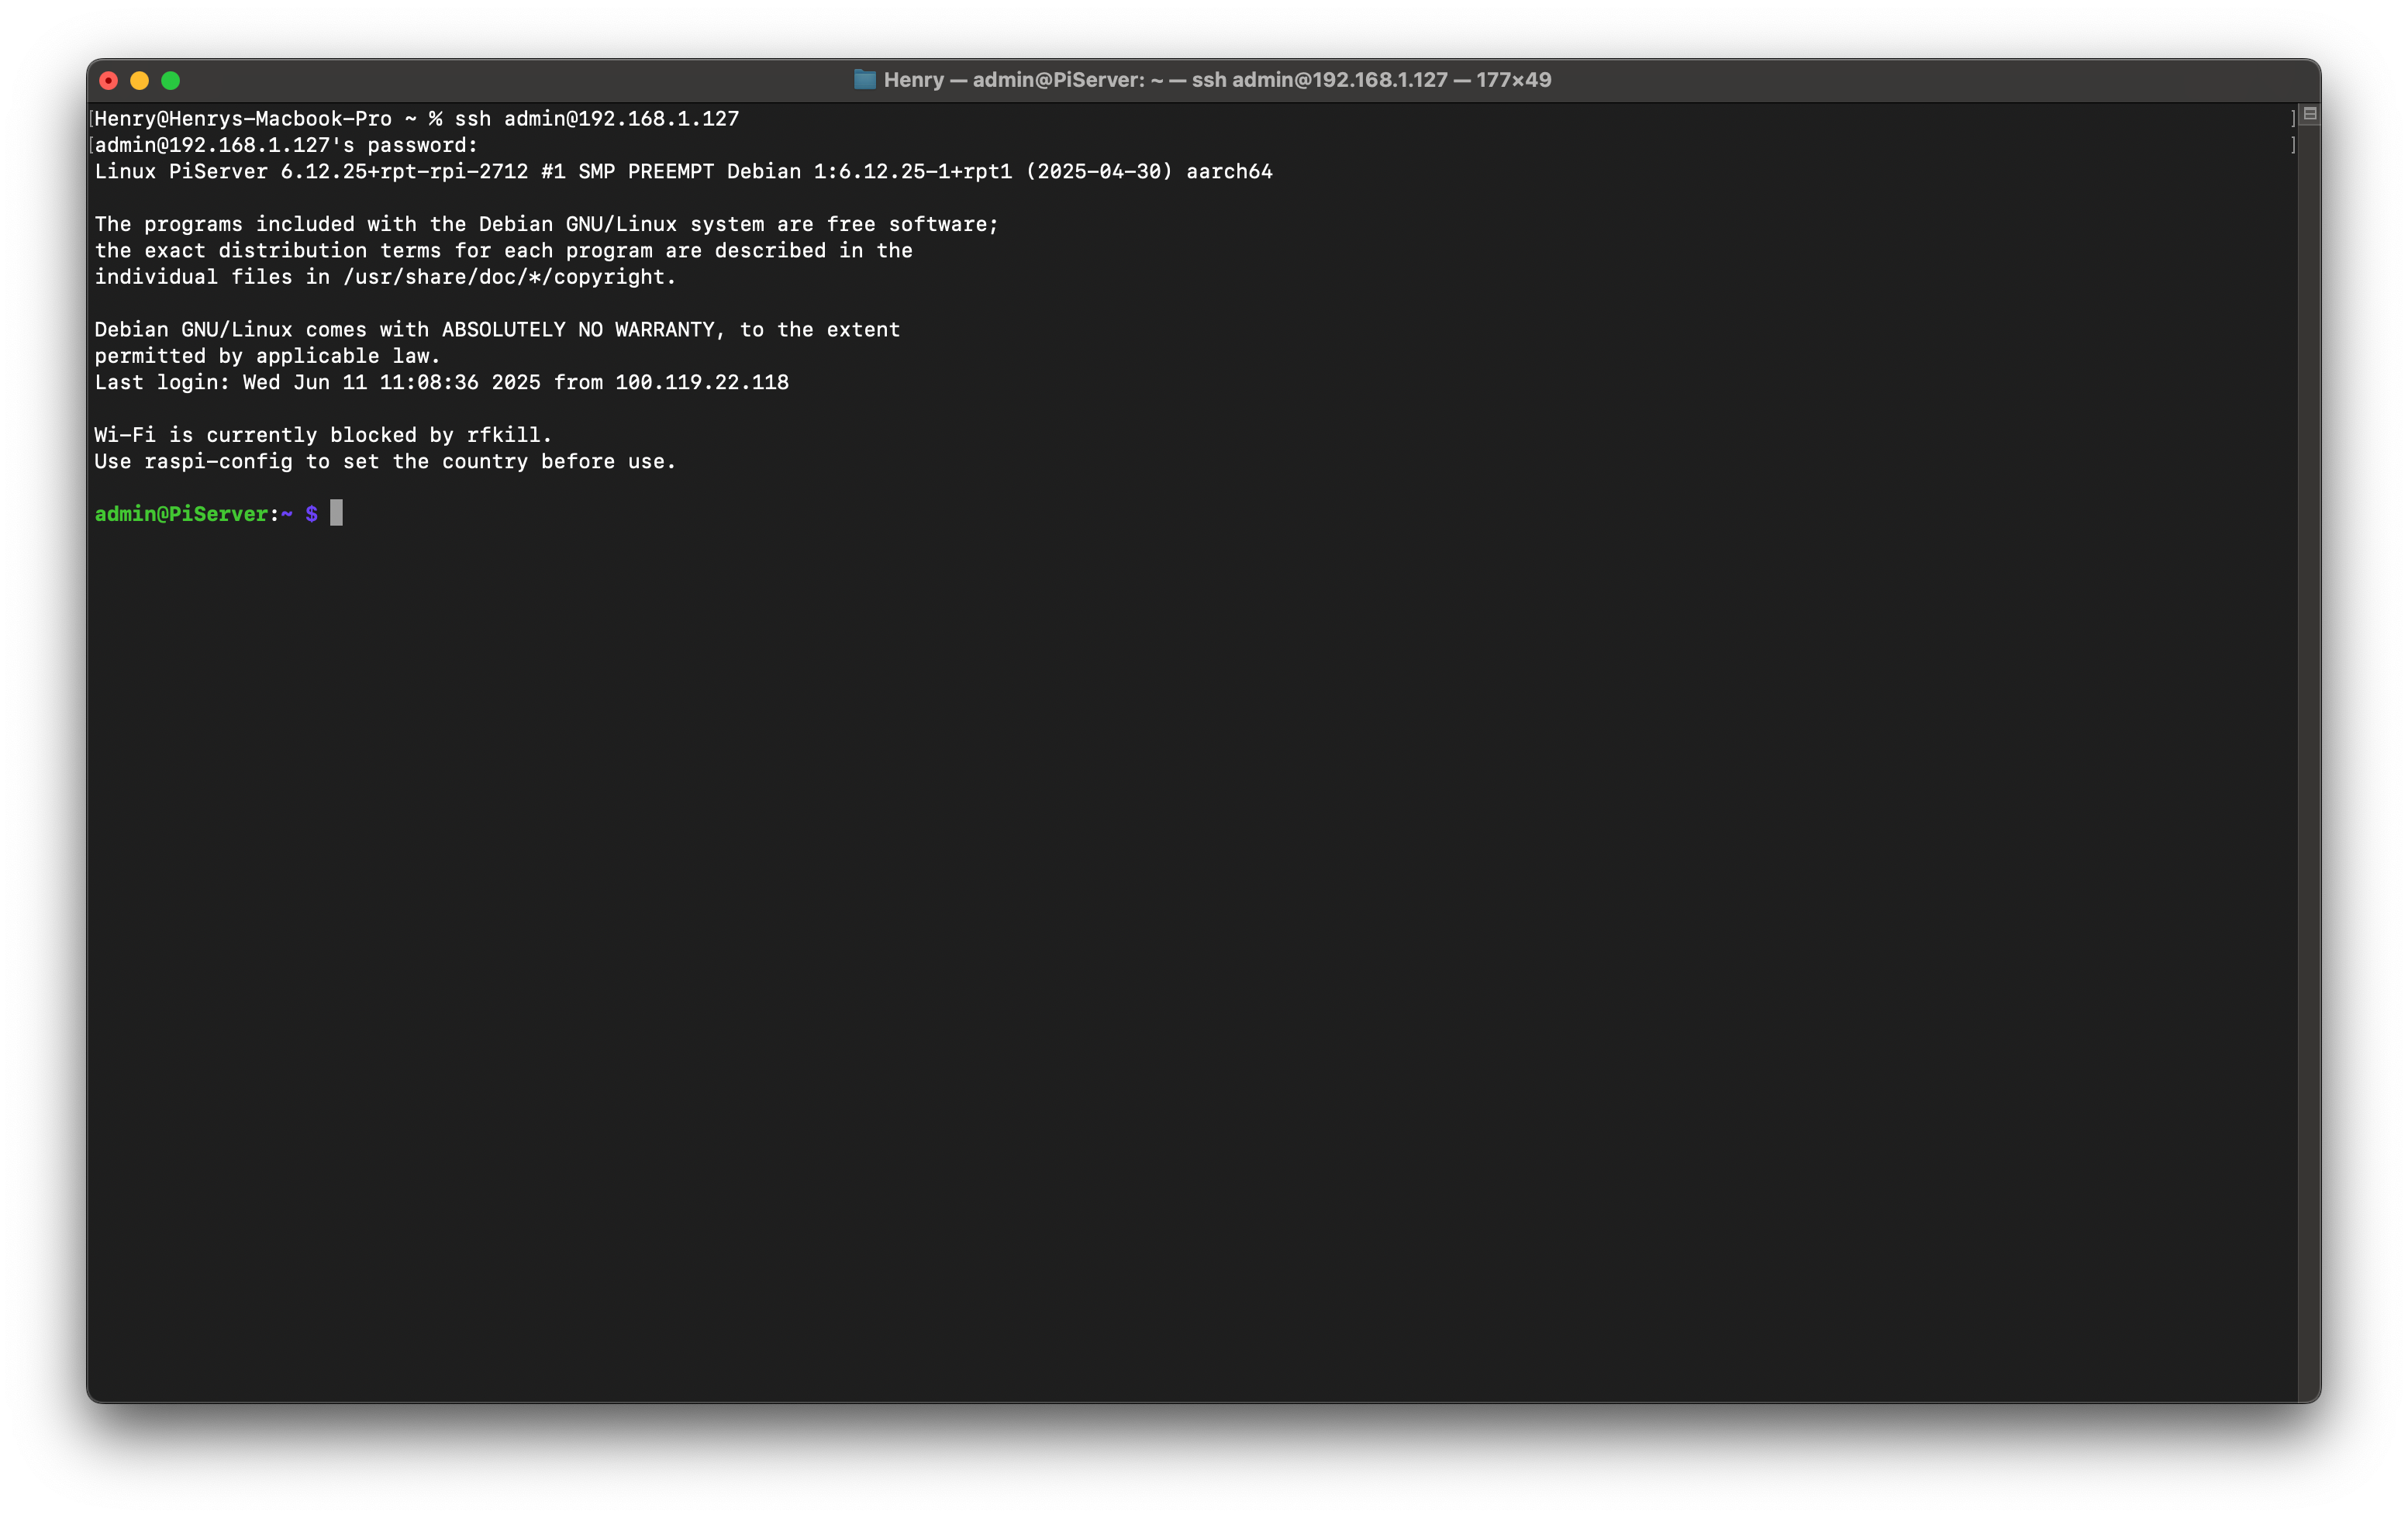
\includegraphics[width=0.8\textwidth]{Research/31_HomeServerDeployment/media/terminalConnection.png}
    \caption{Connectnig to my PI through SSH using the terminal}
\end{figure}


The details surrounding the process of downloading the code to my pi and the challenges I faced can be found in this weeks diary entry

My next challenge is to run the code on my pi reliably 24/7 so that my project is always available. I first started by created a bash script that automatically starts 2 utilities when the pi first receives power (one called Nginx hosts the frontend of my project and one called Gunicorn which handles the backend API), this ensure that should my house have a power cut, as soon as power is restored the project will be running again. By enterprise standards this is not a very good solution and I should have multiple devices around the world running the code (with battery backups) however considering the cost and academic nature of the project I have deemed this uptime (which I will record and reflect on later) to be satisfactory. With these two utilities set up I thought I was done however I faced another challenge. To start each service I would SSH into my pi from my MacBook and run the respective start commands for each, I found though that whenever the terminal session closed on my laptop (either intentionally or through the device sleeping / losing internet etc) the service would stop and result in my project becoming dormant.

To solve this I researched a tool called Tmux which effectively emulates each session as if it was occurring on the pi itself (rather than on my laptop) and allows my device terminal to 'attach' to that session. This means that after my laptop disconnects from the session it remains active and continues to serve traffic and keeping my EPQ online, this also has the benefit of allowing me to split screen the two servers in one SSH connection (rather than two - one for each) and I can connect to that session again at any time, from any device to check the logs and status of each utility.


Currently I can connect to the pi from within my home using the Ip address assigned to it by my local router. Whilst this is great for changing configuration details now I need to have a way of also completing this from outside my home. To achieve this I have done some research into Virtual Private Networks (VPNs). These powerful software tools essentially allow a device to appear as if it is within a local network from anywhere. This means I can be sitting in a coffee shop, connect to my VPN, and take control of my home server as if I was sitting right next to them - a very powerful feature.

In order to make my project accessible to the world at large I in fact use a very similar technology to a VPN called Cloudflare tunnels, this free tool from Cloudflare (one of the largest players in the internet data routing industry) allows anyone to visit the domain I own (henryfield.net) and have each web request they make redirected to a specific device and port on my home network, in this case my pi server. Using this stack of technologies I made my code and software accessible to anyone, anywhere

Finally here are some notes I made during the progress of setting up my server (some details hidden for security reasons):

To conecct on mac: ssh admin@\censor{192.168.1.127}

Acces token for github: \censor{dontworryimnotthatsillyaboutmakingkeyspublic}

git clone https://Nasebyone:@github.com/yourusername/your-private-repo.git

git reset --hard

git pull

python3 -m venv venv

source venv/bin/activate

pip install -r requirements.txt

sudo lsof -i :8000: shows activity on that port

Start tmux session	tmux new -s epq

Detach (leave running)	Ctrl + B, then D

Reattach to it later	tmux attach -t epq

Exit and kill session	exit from both panes

List sessions	tmux ls

Kill session	tmux kill-session -t epq

Startup script: sudo nano /etc/systemd/system/startservers.service

sudo chmod +x /home/admin/start.sh

sudo systemctl daemon-reload

sudo systemctl enable startservers.service

sudo systemctl start startservers.service

CHECK LOGS: sudo journalctl -u startservers.service -f 
